\documentclass{beamer}

\usepackage{listings}
\usepackage[T1]{fontenc}
\usepackage{lmodern}
\usepackage[utf8]{inputenc}


\AtBeginSection
{
  \begin{frame}
    \frametitle{Table of Contents}
    \tableofcontents[currentsection]
  \end{frame}
}

\usepackage{mycolors}
\usecolortheme[named=kaisred]{structure}
\useinnertheme{circles}
\setbeamercolor{frametitle}{fg=kaisred,  bg=kaisgray}
\setbeamercolor{block title example}{bg=white, fg=structure}%


\setbeamertemplate{itemize items}{\textbullet}
% \setbeamertemplate{footline}[text line]{%
%   \parbox{\linewidth}{\vspace*{-8pt}
%     \insertshorttitle\hfill\insertshortauthor\hfill\insertframenumber
%   }
% }
 \setbeamertemplate{navigation symbols}{}



\graphicspath{{./images/}{../images/}}

\definecolor{dkgreen}{rgb}{0,0.6,0}
\definecolor{gray}{rgb}{0.5,0.5,0.5}
\definecolor{mauve}{rgb}{0.58,0,0.82}


\lstdefinestyle{scala}{
  language=scala,
  basicstyle=\scriptsize\ttfamily, 
  breaklines=true,
  keywordstyle=\color{blue},
  commentstyle=\color{dkgreen},
  numbers=left,
  %frame=single, % Border around box
  %numbersep=-7pt,
  numberstyle=\color{gray},
  stringstyle=\color{mauve}
}

\lstdefinestyle{stainless}{
  numbers=none,
  breaklines=true,
  breakautoindent=true,
  breakindent=63pt,
  basicstyle=\footnotesize\ttfamily
}


\begin{document}

\title{Towards Verifying the Bitcoin-S Library}

\author{Ramon Boss, Kai Brünnler, Anna Doukmak}
\institute{Bern University of Applied Sciences}
%\date{2019-06-14}

\frame{\titlepage}


\begin{frame}
  \frametitle{Table of Contents}
  \tableofcontents
\end{frame}


\section{Bitcoin-S}

\begin{frame}[fragile]
  \frametitle{Bitcoin-S}
\begin{lstlisting}[style=scala]
  val privKey = ECPrivateKey.freshPrivateKey
  val spk = P2PKHScriptPubKey(
    pubKey = privKey.publicKey
  )

  val amount = Satoshis(Int64(10000))

  val utxo = TransactionOutput(
    currencyUnit = amount, 
    scriptPubKey = spk
  )

  val tx = BaseTransaction(
    version = Int32.one,
    inputs = List.empty,
    outputs = List(utxo),
    lockTime = UInt32.zero
  )
\end{lstlisting}
\end{frame}




\section{Stainless}


\begin{frame}[fragile]
\frametitle{Stainless: Example}
\begin{lstlisting}[style=scala]
  def factorial(n: Int): Int = {
      require(n >= 0)
      if (n == 0) {
        1
      } else {
        n * factorial(n - 1)
      }
  } ensuring(res => res >= 0)
\end{lstlisting}
\end{frame}



\begin{frame}[fragile]
\frametitle{Stainless: Example}
\begin{block}{Stainless output for the factorial function}
  \medskip
	\centering
		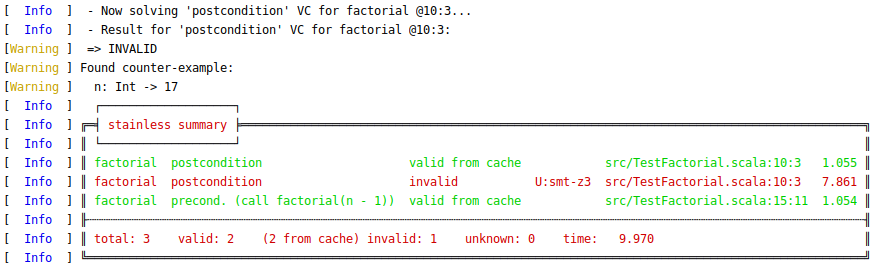
\includegraphics[width=\textwidth]{output1.png}
  \end{block}
\end{frame}

\begin{frame}
\frametitle{Stainless}
\begin{block}{Pure Scala}
\begin{itemize}
  \item Stainless works on a subset of Scala called \emph{Pure Scala}
  \item It's essentially algebraic datatypes (case classes) and pure functions
  \item Some things that it does not include:
    \begin{itemize}
    \item inheritance by objects
    \item abstract type members
    \item inner classes
      in case objects
    \item ...
\end{itemize}

\end{itemize}
\end{block}
\end{frame}


\section{Rewriting Bitcoin-S for Stainless}



\begin{frame}[fragile]
\frametitle{Inheriting Objects}
This:
\begin{lstlisting}[style=scala]
object Satoshis extends BaseNumbers[Satoshis] {
  val zero = Satoshis(Int64.zero)
  val one = Satoshis(Int64.one)
}
\end{lstlisting}

Becomes this:
\begin{lstlisting}[style=scala]
case object Satoshis extends BaseNumbers[Satoshis] {
  val zero = Satoshis(Int64.zero)
  val one = Satoshis(Int64.one)
}
\end{lstlisting}
\end{frame}


\begin{frame}[fragile]
\frametitle{Abstract Type Members}
This:
\begin{lstlisting}[style=scala]
sealed abstract class CurrencyUnit {
  type A

  protected def underlying: A
}

sealed abstract class Satoshis extends CurrencyUnit {
  override type A = Int64
}
\end{lstlisting}

Becomes this:
\begin{lstlisting}[style=scala]
sealed abstract class CurrencyUnit {
  protected def underlying: Int64
}

sealed abstract class Satoshis extends CurrencyUnit
\end{lstlisting}
\end{frame}


\begin{frame}[fragile]
\frametitle{Missing Bitwise \&-Function on BigInt}
This:
\begin{lstlisting}[style=scala]
sealed abstract class Number {
  def andMask: BigInt
  def checkResult(result: BigInt): BigInt = {
    require((result & andMask) == result)
    result
  }
}  
\end{lstlisting}
Becomes this:
\begin{lstlisting}[style=scala]
sealed abstract class Number {
  // removed redundant checkResult function
}
\end{lstlisting}
\end{frame}


\begin{frame}[fragile]
\frametitle{Specification and Stainless Output}
\begin{lstlisting}[style=scala]
def +(c: CurrencyUnit): CurrencyUnit = {
  require(c.satoshis == Satoshis.zero)
  Satoshis(
    satoshis.underlying + c.satoshis.underlying
  )
} ensuring(res => res.satoshis == this.satoshis)
\end{lstlisting}

\bigskip\bigskip

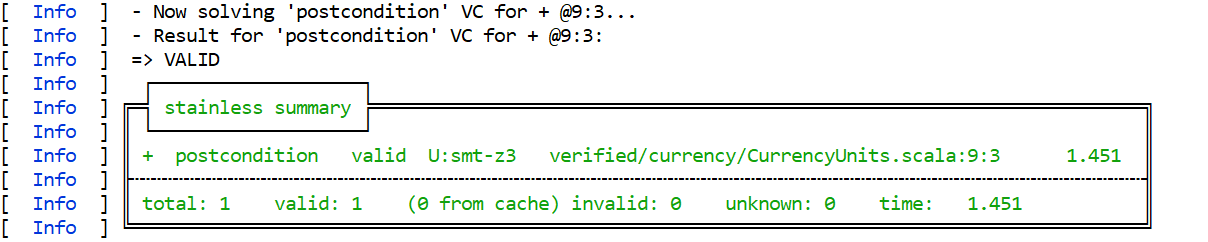
\includegraphics[width=\textwidth]{result_output}
\end{frame}



\section{Bugs We Found}


\begin{frame}
\frametitle{Bug 1: Function checkTransaction is too restrictive}
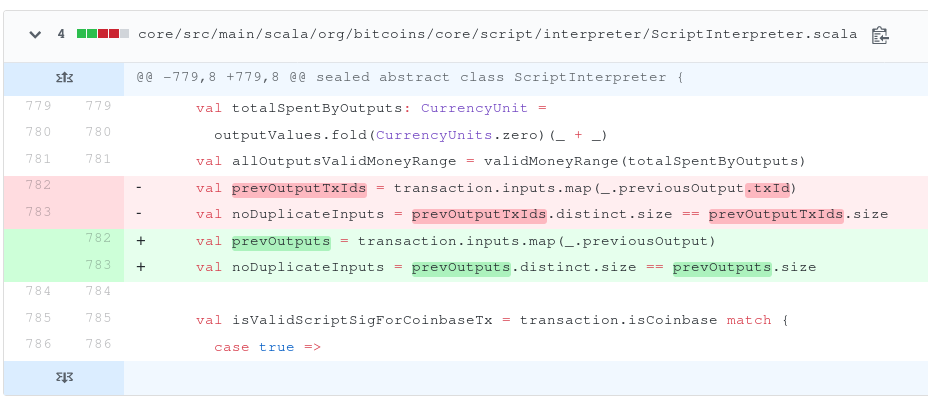
\includegraphics[width=\textwidth]{bug1.png}
\end{frame}

\begin{frame}
\frametitle{Bug 2: Function checkResult is buggy (and redundant)}
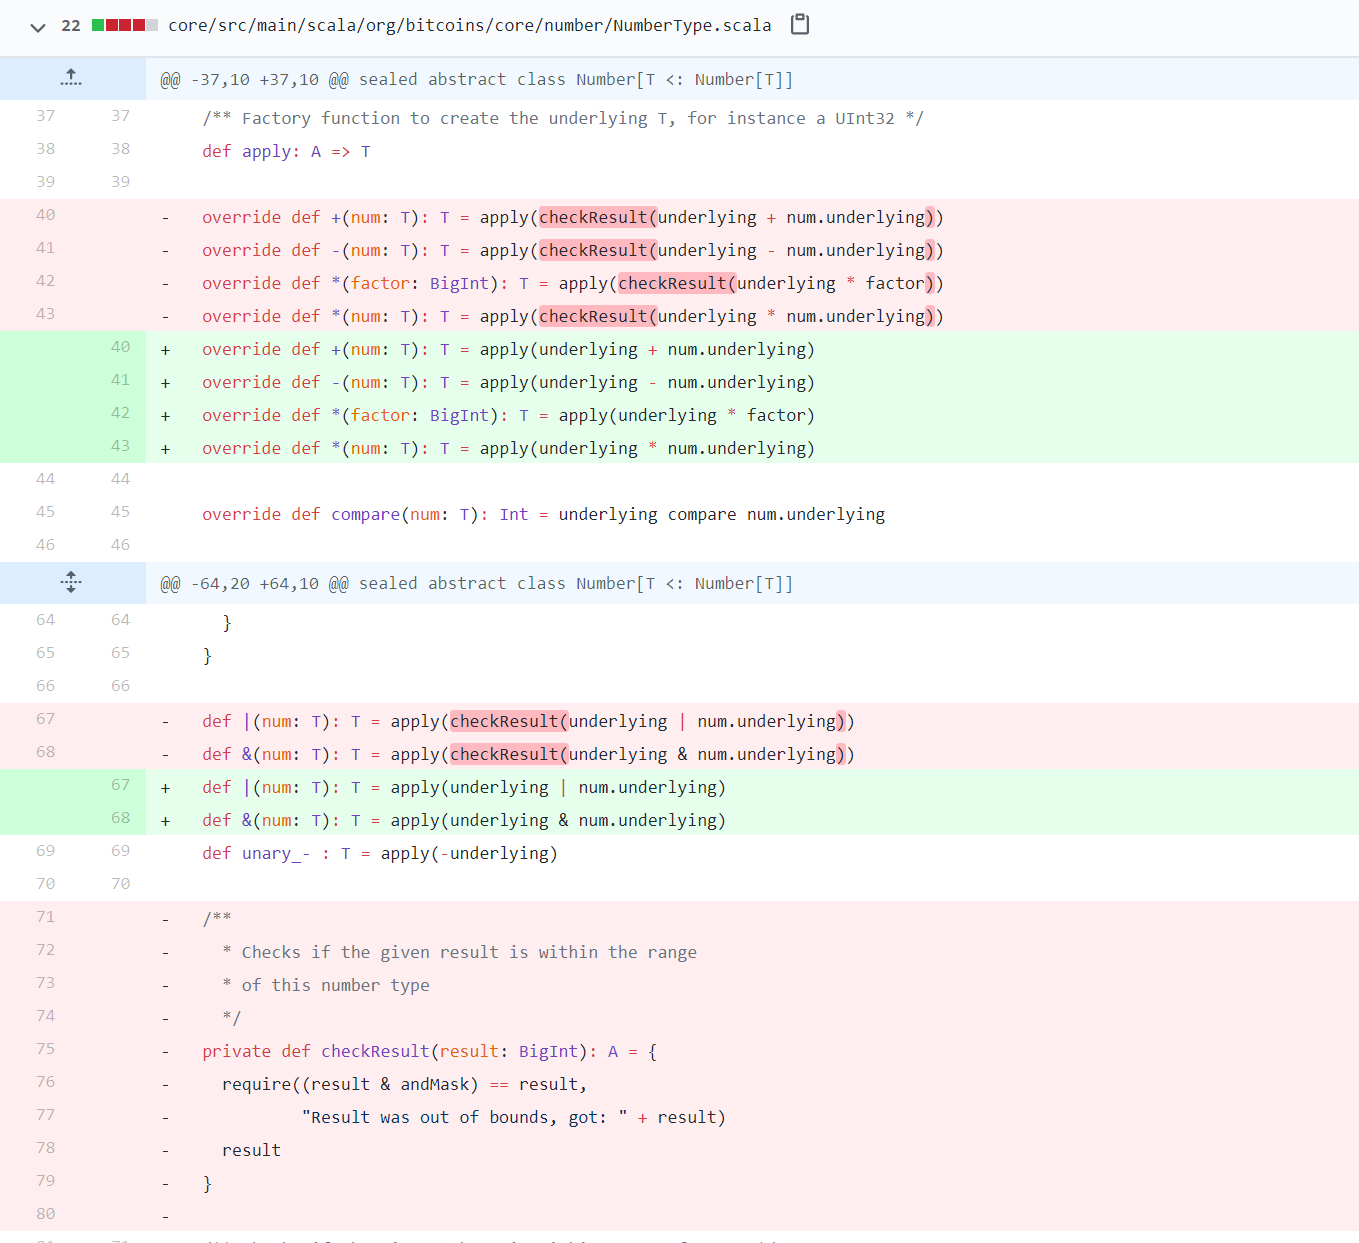
\includegraphics[width=.85\textwidth]{bug2.png}
\end{frame}

\begin{frame}
\frametitle{Conclusion}
\begin{block}{Lessons learned}
  \begin{itemize}
  \item Even verifying very simple properties requires significantly rewriting existing Scala code
  \item This is true even for purely functional code
  \item We can't really verify existing code -- really we verify a re-implementation of it
  \item But attempting to verify has been very useful for finding bugs
  \end{itemize}
\end{block}

\end{frame}

\end{document}
